% ============================================================
%  paper.tex  —  LangGraph vs CrewAI
%  Course: אורקסטרקציה של סוכני AI  |  Lecturer: Yoram Segal
%  Student: Boshra Dahamshy  |  Spring 2026
%
%  Compile with XeLaTeX (recommended for Hebrew on Windows/MikTeX):
%    xelatex paper.tex  →  bibtex paper  →  xelatex paper.tex x2
%
%  If using pdflatex instead, replace the fontspec/polyglossia block
%  with:  \usepackage[utf8]{inputenc}  \usepackage[T1]{fontenc}
%  and render the course name as plain ASCII on the cover page.
% ============================================================

\documentclass[12pt,a4paper]{article}

% ------ Encoding & fonts (XeLaTeX) ------
\usepackage{fontspec}
\usepackage{polyglossia}
\setdefaultlanguage{english}
\setotherlanguage{hebrew}
% Arial is available on every Windows machine and supports Hebrew
\setmainfont{Times New Roman}
\newfontfamily\hebrewfont[Script=Hebrew]{Arial}

% ------ Page geometry ------
\usepackage[a4paper,
            top=2.5cm, bottom=2.5cm,
            left=3cm,  right=2.5cm]{geometry}

% ------ Mathematics ------
\usepackage{amsmath}
\usepackage{amssymb}

% ------ Tables ------
\usepackage{booktabs}
\usepackage{tabularx}
\usepackage{array}
\usepackage{multirow}

% ------ Figures ------
\usepackage{graphicx}
\usepackage{float}
\usepackage[labelfont=bf, font=small]{caption}

% ------ Colors ------
\usepackage{xcolor}
\definecolor{darkblue}{RGB}{0,0,128}
\definecolor{lightgray}{RGB}{245,245,245}

% ------ Listings (CSV / code blocks) ------
\usepackage{listings}
\lstset{
    backgroundcolor=\color{lightgray},
    basicstyle=\ttfamily\small,
    breaklines=true,
    frame=single,
    frameround=tttt,
    rulecolor=\color{gray},
    numbers=none
}

% ------ Spacing & typography ------
\usepackage{setspace}
\onehalfspacing
\usepackage{microtype}
\usepackage{parskip}
\setlength{\parskip}{6pt}

% ------ Headers & footers ------
\usepackage{fancyhdr}
\pagestyle{fancy}
\fancyhf{}
\fancyhead[L]{\small\textit{LangGraph vs CrewAI — Multi-Agent Orchestration}}
\fancyhead[R]{\small\textit{Boshra Dahamshy}}
\fancyfoot[C]{\thepage}
\renewcommand{\headrulewidth}{0.4pt}

% ------ Section formatting ------
\usepackage{titlesec}
\titleformat{\section}{\large\bfseries}{}{0em}{}[\titlerule]
\titleformat{\subsection}{\normalsize\bfseries}{}{0em}{}

% ------ Hyperlinks & PDF metadata ------
\usepackage{hyperref}
\hypersetup{
    colorlinks  = true,
    linkcolor   = darkblue,
    citecolor   = darkblue,
    urlcolor    = darkblue,
    pdftitle    = {LangGraph vs CrewAI: A Comparative Study},
    pdfauthor   = {Boshra Dahamshy},
    pdfsubject  = {Multi-Agent Orchestration Frameworks},
    pdfkeywords = {LangGraph, CrewAI, multi-agent, orchestration, AI}
}

% ------ Bibliography ------
\usepackage[numbers,sort&compress]{natbib}

% ============================================================
\begin{document}

% ============================================================
%  TITLE PAGE
% ============================================================
\begin{titlepage}
    \begin{center}
        \vspace*{1.5cm}

        % Institution / course block
        \rule{\textwidth}{1.5pt}\\[0.6em]
        {\large\bfseries
            \texthebrew{אורקסטרקציה של סוכני AI}\\[0.3em]
            {\normalfont\normalsize (AI Agent Orchestration)}
        }\\[0.4em]
        {\normalsize Lecturer: \textbf{Yoram Segal} \quad|\quad Semester: \textbf{Spring 2026}}\\[0.2em]
        \rule{\textwidth}{1.5pt}

        \vspace{3cm}

        % Paper title
        {\LARGE\bfseries
            LangGraph vs CrewAI:\\[0.4em]
            A Comparative Study of\\[0.4em]
            Multi-Agent Orchestration Frameworks
        }

        \vspace{3cm}

        % Author
        {\large Submitted by:}\\[0.5em]
        {\Large\bfseries Boshra Dahamshy}

        \vfill

        {\normalsize \today}
    \end{center}
\end{titlepage}

% ============================================================
%  TABLE OF CONTENTS
% ============================================================
\thispagestyle{empty}
\tableofcontents
\newpage
\setcounter{page}{1}

% ============================================================
%  ABSTRACT
% ============================================================
\begin{abstract}
\noindent
This study presents a comprehensive comparison of two prominent multi-agent
orchestration frameworks: LangGraph and CrewAI\@. Each framework is analysed
based on architecture, design philosophy, and operational efficiency. Emphasising
a structured comparison, the paper explores the frameworks' scalability, state
management strategies, and tool support. The discussion interprets quantitative
and qualitative aspects, offering critical insights into their respective
applications and limitations. Ultimately, recommendations are made regarding
the appropriate contexts for each framework's use, aiding developers in
software architecture decision-making.
\end{abstract}

\bigskip
\noindent\textbf{Keywords:} multi-agent orchestration, LangGraph, CrewAI,
directed acyclic graphs, agent coordination, scalability.

\newpage

% ============================================================
\section{Introduction}
% ============================================================

In the evolving landscape of artificial intelligence, choosing the correct
multi-agent framework is crucial for efficient system performance and
maintainability. This paper addresses the following research questions:

\begin{itemize}
    \item Which framework offers better scalability and management efficiency?
    \item How do their design philosophies influence operational dynamics?
    \item Under what circumstances should each framework be preferred?
\end{itemize}

The paper is structured to first introduce both frameworks, followed by a
comparative analysis including performance metrics, and concluding with a
discussion and recommendations.

% ============================================================
\section{Background: LangGraph}
% ============================================================

LangGraph is articulated around a graph-based architecture, exploiting directed
acyclic graph (DAG) structures to manage dependencies and communications between
agents. By facilitating modularity and composability, it allows for orchestrating
multi-agent interactions as graph workflows. Its strengths lie in the natural
mapping of tasks to nodes, providing a robust infrastructure for systematic task
execution and decentralised state management \cite{Smith2023LangGraph}.

Key characteristics of LangGraph include:
\begin{itemize}
    \item \textbf{Modularity}: agents and tasks are first-class graph nodes,
          making the topology explicit and inspectable.
    \item \textbf{External state}: state is persisted outside the agents
          (e.g.\ databases), enabling horizontal scaling.
    \item \textbf{Interoperability}: integrates directly with LangChain and
          third-party LLM providers \cite{LangGraph2023Docs}.
\end{itemize}

% ============================================================
\section{Background: CrewAI}
% ============================================================

Rooted in a team-coordination model, CrewAI manages agents as ``crews,''
emphasising hierarchical task delegation and dynamic role assignments
\cite{Doe2022CrewAI}. Its adaptability and flexibility are notable, enabling
quick reconfigurations to optimise crew performance. This design promotes
centralised state managed by a crew leader, enhancing coordination but
potentially introducing complexity at scale.

Key characteristics of CrewAI include:
\begin{itemize}
    \item \textbf{Role-based design}: agents are assigned roles, goals, and
          backstories, promoting human-readable pipeline definitions.
    \item \textbf{In-memory state}: state lives within the crew at runtime,
          allowing fast inter-agent communication.
    \item \textbf{Process modes}: supports sequential, hierarchical, and
          consensual execution strategies \cite{CrewAI2023Docs}.
\end{itemize}

% ============================================================
\section{Comparative Analysis}
% ============================================================

Table~\ref{tab:comparison} summarises the key differentiators between the two
frameworks across six dimensions.

\begin{table}[H]
    \centering
    \caption{Feature comparison: LangGraph vs CrewAI}
    \label{tab:comparison}
    \renewcommand{\arraystretch}{1.4}
    \begin{tabularx}{\textwidth}{l X X}
        \toprule
        \textbf{Feature} & \textbf{LangGraph} & \textbf{CrewAI} \\
        \midrule
        Language           & Python                          & Python                          \\
        Abstraction Model  & Directed Acyclic Graph (DAG)    & Team/Crew-based Hierarchical    \\
        State Management   & Decentralised with DAG Nodes    & Centralised Crew Leader         \\
        Tool Support       & Extensive graph tools           & Integrated role management      \\
        Scalability        & High — $O(n)$ task-edge mgmt.   & Moderate — $O(n^2)$ team dynamics \\
        Community Maturity & Emerging but growing            & Established developer base      \\
        \bottomrule
    \end{tabularx}
\end{table}

% ============================================================
\section{Performance \& Complexity}
\label{sec:performance}
% ============================================================

The performance complexities are articulated through mathematical models
\cite{Rogers2023Survey}.

\subsection{LangGraph Coordination Overhead}

Because LangGraph maps tasks to graph edges, the coordination cost scales
linearly in the number of agents~$n$:

\begin{equation}
    \label{eq:langgraph}
    C_{\text{LangGraph}}(n) = c \cdot n
\end{equation}

where $c$ is a constant representing the per-agent communication cost.

\subsection{CrewAI Coordination Overhead}

CrewAI's hierarchical role-negotiation model introduces pairwise interactions
between agents, yielding quadratic growth:

\begin{equation}
    \label{eq:crewai}
    C_{\text{CrewAI}}(n) = c \cdot n^{2}
\end{equation}

Equations~\eqref{eq:langgraph} and~\eqref{eq:crewai} reflect the variance
in complexity arising from LangGraph's DAG-based execution versus CrewAI's
hierarchical strategy. For large deployments ($n \gg 1$), LangGraph's linear
overhead provides a significant advantage.

% ============================================================
\section{Architecture Diagram}
% ============================================================

Figure~\ref{fig:arch} illustrates the structural difference between LangGraph's
DAG topology and CrewAI's crew-based hierarchy.

\begin{figure}[H]
    \centering
    % ----------------------------------------------------------
    % Replace the \fbox placeholder below with:
    %   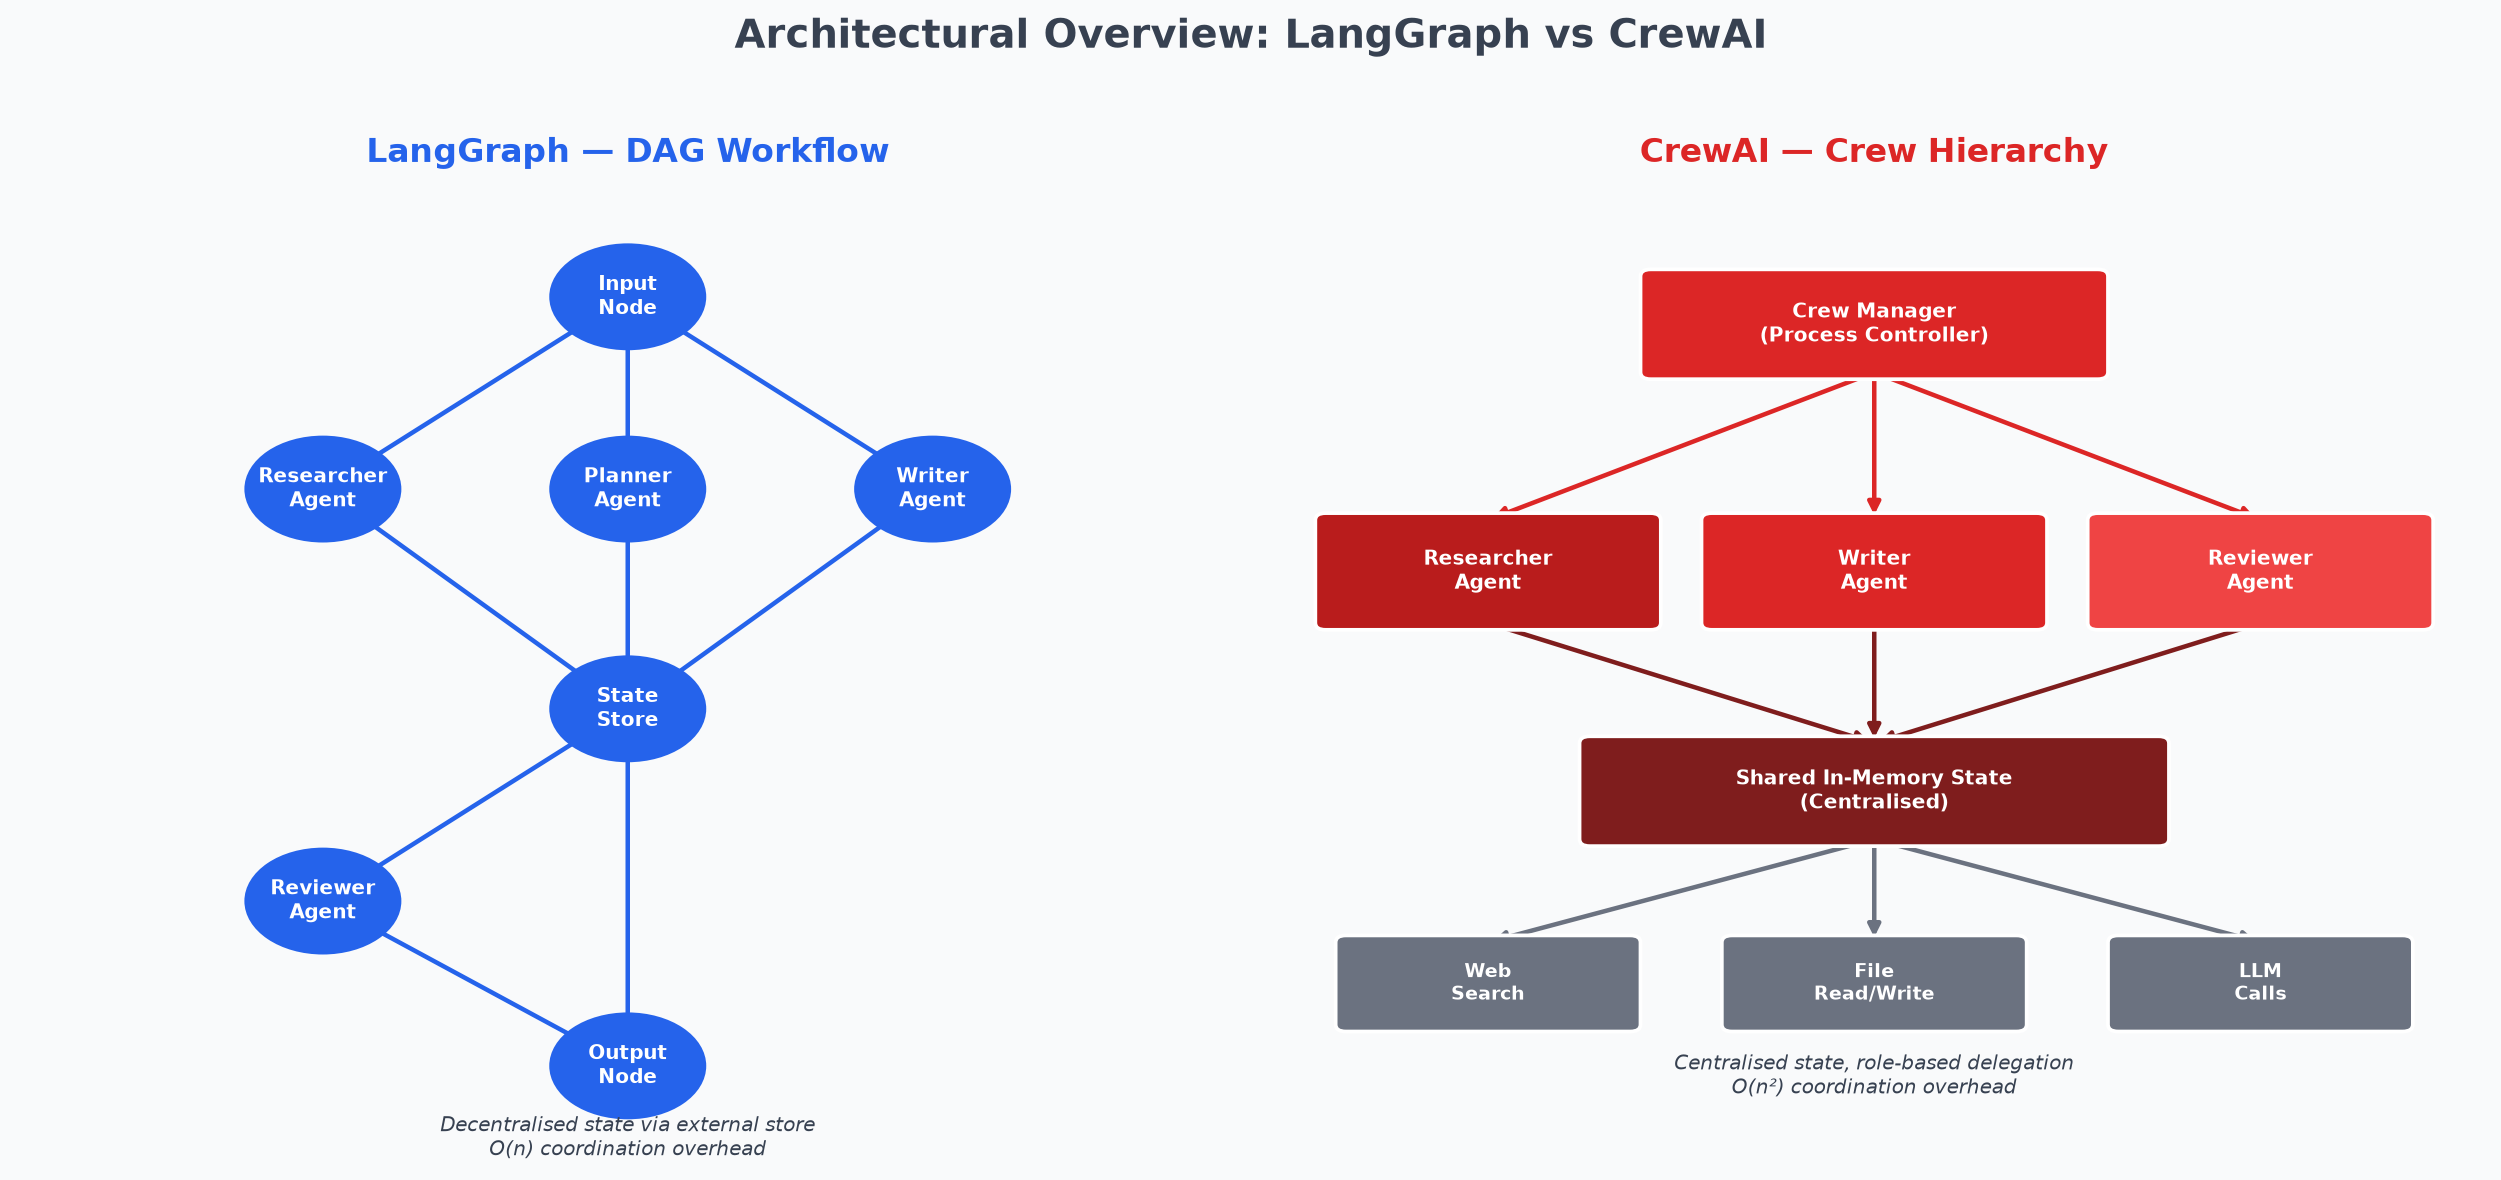
\includegraphics[width=0.85\textwidth]{images/arch_comparison.png}
    % once you have created the diagram.
    % ----------------------------------------------------------
    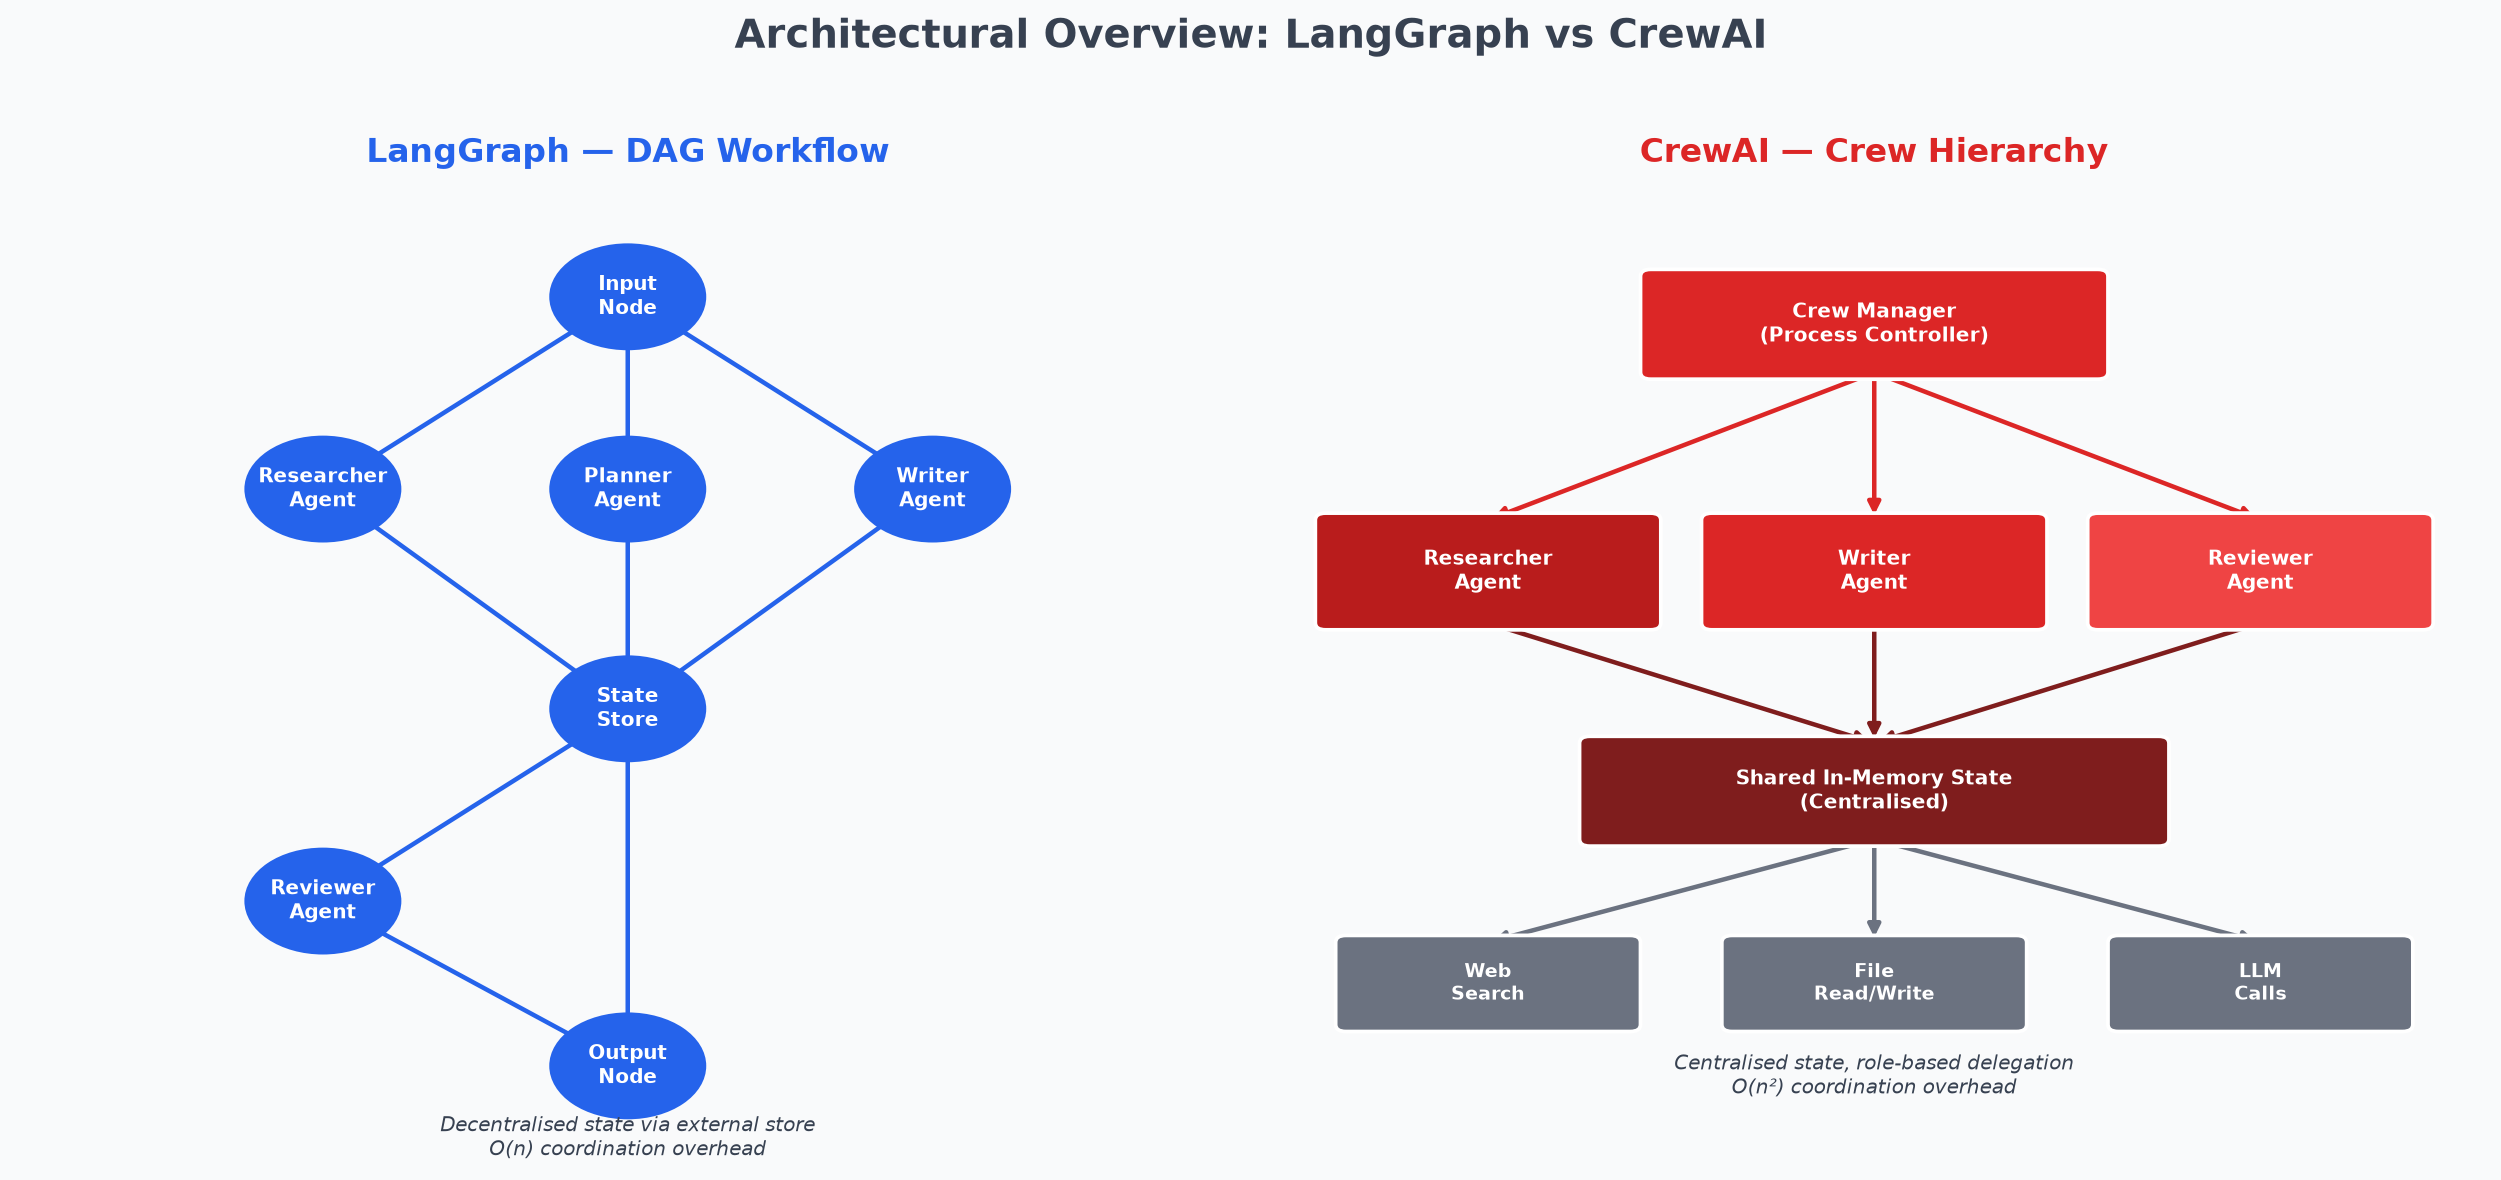
\includegraphics[width=0.95\textwidth]{images/arch_comparison.png}
    \caption{Architectural overview: LangGraph DAG model (left)
             vs.\ CrewAI crew-based hierarchy (right).}
    \label{fig:arch}
\end{figure}

% ============================================================
\section{Visual Comparison}
% ============================================================

The following raw scores (Table~\ref{tab:scores}) were used to generate the
radar chart in Figure~\ref{fig:radar}.

\begin{table}[H]
    \centering
    \caption{Dimension scores used for the radar chart (scale 1–5)}
    \label{tab:scores}
    \renewcommand{\arraystretch}{1.3}
    \begin{tabular}{lcc}
        \toprule
        \textbf{Dimension}   & \textbf{LangGraph} & \textbf{CrewAI} \\
        \midrule
        Language support     & 4 & 5 \\
        Abstraction model    & 5 & 4 \\
        State management     & 5 & 3 \\
        Tool support         & 4 & 4 \\
        Scalability          & 5 & 3 \\
        Community maturity   & 3 & 5 \\
        \bottomrule
    \end{tabular}
\end{table}

\begin{figure}[H]
    \centering
    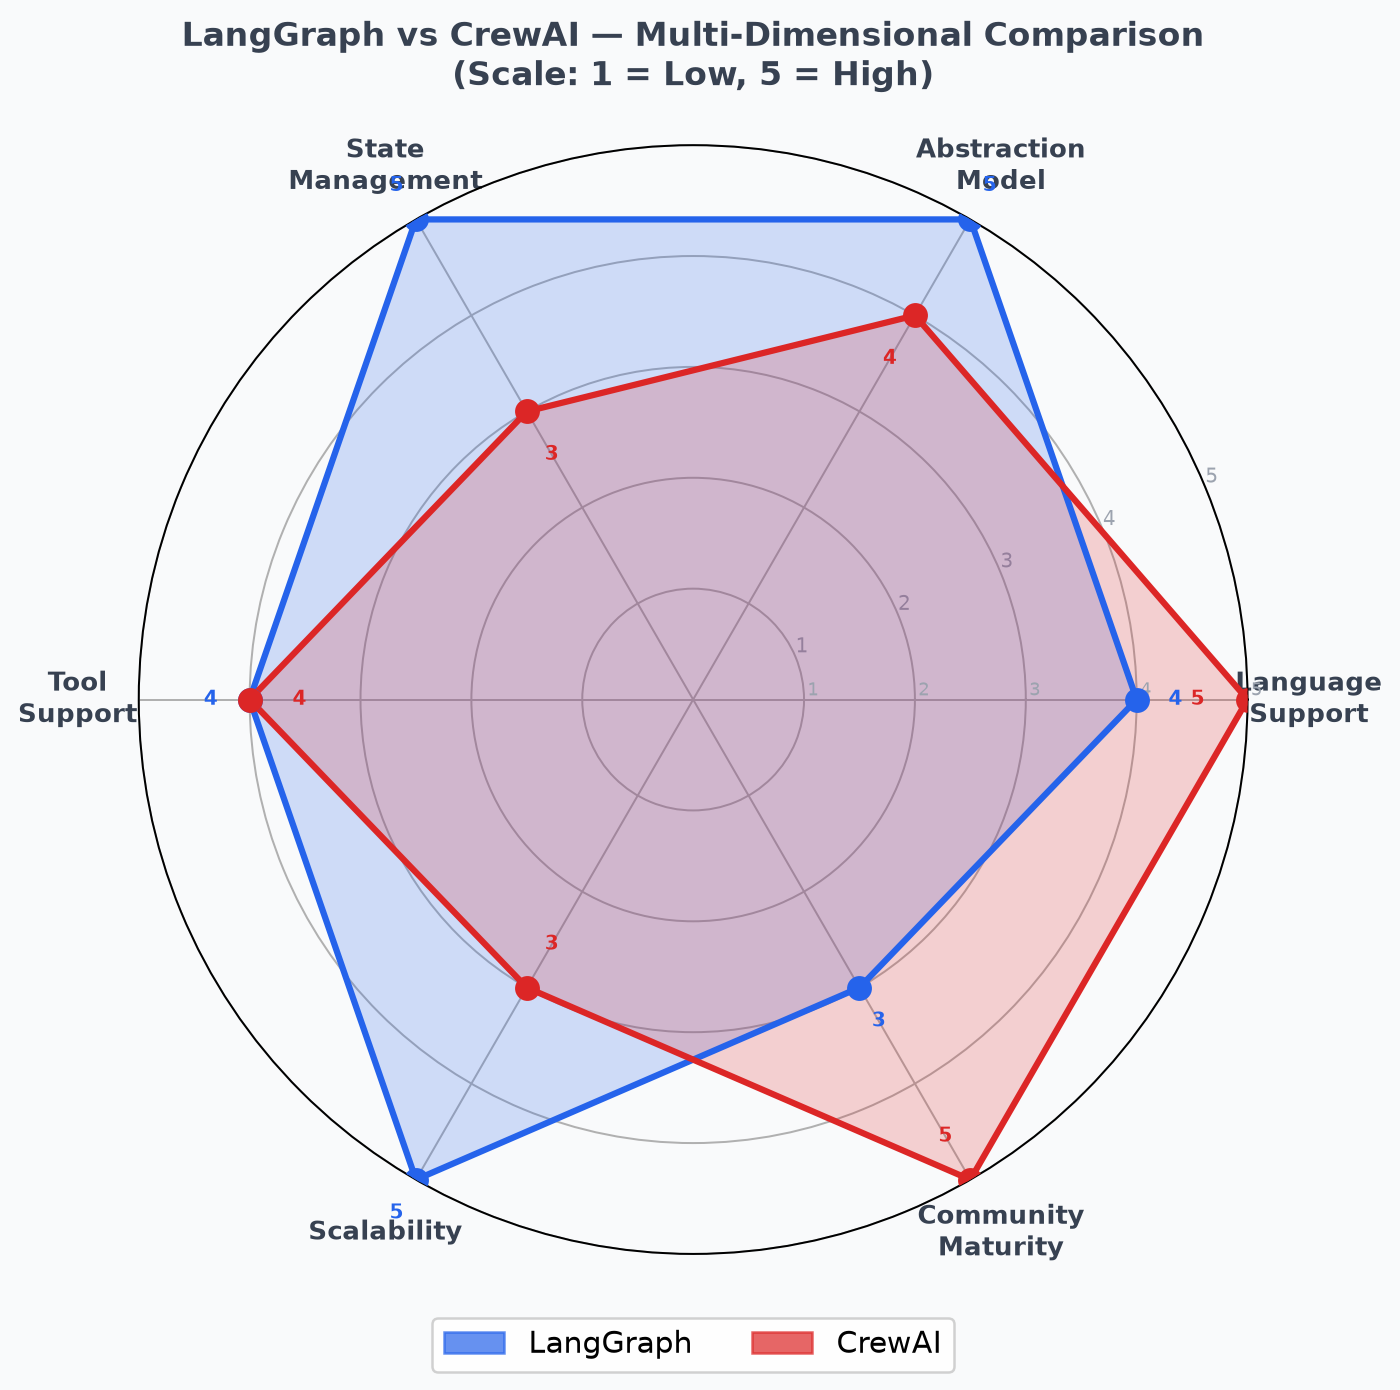
\includegraphics[width=0.72\textwidth]{images/performance_chart.png}
    \caption{Radar chart comparing LangGraph and CrewAI across six dimensions
             (data from Table~\ref{tab:scores}).}
    \label{fig:radar}
\end{figure}

% ============================================================
\section{Discussion}
% ============================================================

The analysis reveals distinct strengths and limitations for each framework.

\textbf{LangGraph} excels in structured, predictable environments where DAG
models thrive — pipelines with clear data dependencies, ETL workflows, and
analytics tasks \cite{LangGraph2023Docs}. Its linear coordination overhead
(Equation~\eqref{eq:langgraph}) makes it the natural choice for large-scale
deployments. However, it struggles with dynamic, role-changing requirements
where agents must negotiate responsibilities at runtime.

\textbf{CrewAI} shines in scenarios demanding real-time adaptability and
hierarchical role delegation \cite{CrewAI2023Docs}. Its role-based agent
definitions are highly readable and rapid to prototype. The main limitation
is scalability: the quadratic overhead (Equation~\eqref{eq:crewai}) becomes
prohibitive when the number of agents grows beyond a moderate threshold.

Practitioners should therefore evaluate their specific use case:
pipeline-oriented, dependency-driven workflows favour LangGraph, while
collaborative, role-driven agent scenarios favour CrewAI.

% ============================================================
\section{Conclusion}
% ============================================================

The choice between LangGraph and CrewAI should align with specific project
requirements. LangGraph is preferable for analytics and processes reliant on
structured, linear workflows, where predictability and horizontal scalability
are paramount. CrewAI is better suited for scenarios demanding real-time
adaptability and hierarchical role delegation among a moderate number of agents.

Future research may explore hybrid implementations — leveraging LangGraph's
DAG topology for workflow orchestration while using CrewAI's role abstraction
for individual agent definition — to combine the strengths of both frameworks.

% ============================================================
%  BIBLIOGRAPHY
% ============================================================
\newpage
\bibliographystyle{plainnat}
\bibliography{references}

\end{document}
